\section{ТЕСТИРОВАНИЕ}
    \subsection{Статический анализ}
    % TODO Статический анализ
    Для статического анализа соответствия типов в Python используются аннотации 
    из встроенного модуля \inlinecode{typing} и специальный линтер и анализатор.
    Существует несколько анализаторов,
    и \textit{mypy}\cite{mypy} - наиболее популярный из них.
    Он полностью написан на Python, поддерживается и развивается открытым
    сообществом 
    и Гвидо ван Россумом (\textit{Guido van Rossum} \cite{guido.van.rossum})
    в частности. Поэтому проект быстрее получает поддержку новых изменений в
    синтаксисе языка, что особенно важно для нас, так как в проекте на данный
    момент используются последняя мажорная версия Python 3.8.

    Так как многие Python сторонние библиотеки уже написаны без использования
    аннотации типов, их дополняют заголовочными модулями,
    так называемыми \textit{stub}-файлами. В таком случае, статическую типизацию
    можно использовать даже с изначально динамически типизированными модулями.
    
    \textit{Mypy} может использоваться как консольная утилита, подсказывая ошибки в
    использовании переменных и функций, но также может генерировать полноценные
    отчеты, как на примере ниже.
    \begin{figure}[H]
        \centering
        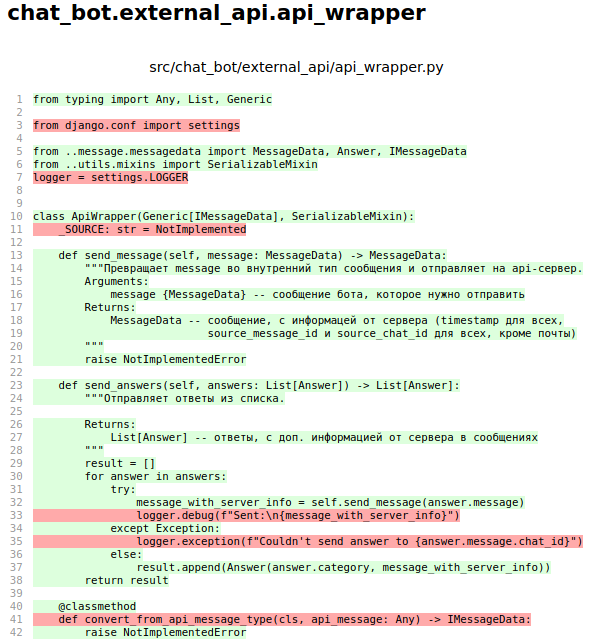
\includegraphics[width=\linewidth]{static/mypy-report.png}
        \caption{Отчет \textit{mypy} в формате html}
        \label{fig:mypy-report}
    \end{figure}
    
    \subsection{Юнит-тесты}
    % TODO Юнит-тесты

    \subsection{Нагрузочное тестирование}
    Нагрузочное тестирование проводилось на тестовом сервере на полностью
    развернутом веб-приложении с веб-сервером \textit{Nginx} при помощи
    инструмента Яндекс.Танк. Целью нагрузочного тестирования было установление
    порога стабильной работы сервиса, для этого на него подавалась нагрузка
    с константным количеством запросов в секунду в течение 2 минут с итеративным
    увеличением количества запросов.

    Так, был составлен следующий конфигурационный файл для Яндекс.Танка:
    \begin{figure}[H]
        \centering
        \lstinputlisting[language=Python]{snippets/load.yaml}
        \caption{Конфигурационный файл Яндекс.Танка}
        \label{fig:tank_load}
    \end{figure}

    Так, было установлено, что сервис стабильно выдерживает нагрузку до 18
    запросов в секунду в течение 2 минут.
    % TODO какой-нибудь график
